\section{Results}
\subsection{Populations reconstructed at 50 MeV}
The central cosmological input fixed $Y_{\Delta B}^{\rm ref}=8.69318\times10^{-11}$. With this same excess per entropy unit, the PDG2025 HRG at 50 MeV ($5.8023\times10^{11}$ K) yielded $n_B=2.7261\times10^{30}$ and $n_{\bar B}=2.7172\times10^{30}$ cm$^{-3}$. The sum was $5.4433\times10^{30}$ cm$^{-3}$ and the net excess was $8.8765\times10^{27}$ cm$^{-3}$ (Table~\ref{tab:states}). These four values are results of the inverse calculation; the net yield was the imposed external condition.

The ratio $R=306.1147$ means that approximately 306.1 antibaryons and 307.1 baryons coexisted per unit of net excess in this state. The ratio $n_{\bar B}/n_B=0.996744$ was obtained: approximately 99.6744 antibaryons per 100 baryons. The excess represented 0.163071\% of the sum. The solution required $\mu_B/T=0.00163071$, equivalent to $\mu_B=0.0815356$ MeV.

\begin{table*}[t]\centering\small
\caption{Reconstructed PDG2025 states at the central input $\eta$. Densities refer to physical volume at each temperature; $R=n_{\bar B}/\Delta n_B$.}
\label{tab:states}
\setlength{\tabcolsep}{6pt}
\begin{tabular}{rrrrrr}\toprule
$T$ (MeV) & $n_B$ (cm$^{-3}$) & $n_{\bar B}$ (cm$^{-3}$) & $\Delta n_B$ (cm$^{-3}$) & $R$ & $\mu_B/T$\\\midrule
50.0 & $2.7261\times10^{30}$ & $2.7172\times10^{30}$ & $8.8765\times10^{27}$ & 306.114688 & 0.001631\\
45.0 & $2.8323\times10^{29}$ & $2.7694\times10^{29}$ & $6.2899\times10^{27}$ & 44.028849 & 0.011229\\
40.0 & $1.9166\times10^{28}$ & $1.4894\times10^{28}$ & $4.2724\times10^{27}$ & 3.486095 & 0.126100\\
38.203739 & $7.3454\times10^{27}$ & $3.6727\times10^{27}$ & $3.6727\times10^{27}$ & 1.000000 & 0.346574\\
37.0 & $4.4167\times10^{27}$ & $1.1116\times10^{27}$ & $3.3051\times10^{27}$ & 0.336326 & 0.689799\\
\bottomrule\end{tabular}
\end{table*}


Protons, neutrons, and their antiparticles contributed 95.2176\% of the total baryonic population at 50 MeV; the other catalog baryons contributed 4.7824\%. Table~\ref{tab:nucleons50} identifies the nucleon contributions with their retained rest masses. The entropy fraction of the baryon-antibaryon sector was $s_{B+\bar B}/s_{\rm tot}=1.15182\times10^{-6}$; this entropy fraction differs from a fraction of particle number.

\begin{table}[t]\centering\small
\caption{Nucleons and their antiparticles at 50 MeV, PDG2025. Density is given in units of $10^{30}$ cm$^{-3}$.}
\label{tab:nucleons50}
\begin{tabular}{lrr}\toprule
Particle species & Mass (MeV) & Density\\\midrule
$p$ & 938.272 & 1.313384\\
$\bar p$ & 938.272 & 1.309107\\
$n$ & 939.565 & 1.282334\\
$\bar n$ & 939.565 & 1.278159\\
\bottomrule\end{tabular}
\end{table}


\subsection{Thermal sequence and abundance crossing}
As temperature decreased from 50 to 45 and 40 MeV, $R$ decreased from 306.1147 to 44.02885 and 3.486095. At the published temperature of 38.2 MeV, $R=0.997012$ was obtained; the independently calculated root was $T_\times=38.203739$ MeV (Figure~\ref{fig:cross}). The crossing rounds to 38.2 MeV at the precision reported by \citet{Yang2022}. The arithmetic difference, $+0.003739$ MeV, does not provide a statistical precision for the agreement.

At the PDG2025 root, $n_{\bar B}=\Delta n_B=3.6727\times10^{27}$ cm$^{-3}$ and $n_B=7.3454\times10^{27}$ cm$^{-3}$. By definition, $R=1$ implies $n_B=2n_{\bar B}$, $n_{\bar B}/n_B=1/2$, and an excess equal to one third of the sum. Antibaryons were still present at this reference point. The nucleon contribution reached 98.8254\%.

\begin{figure*}[t]
\centering
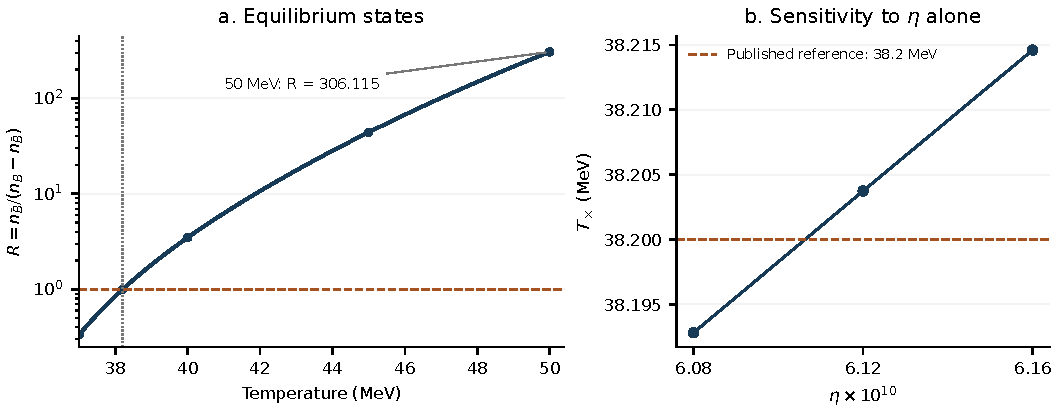
\includegraphics[width=.98\textwidth]{figures/final_cross_en.pdf}
\caption{Antibaryon-to-net-excess ratio for PDG2025. Left: sequence of equilibrium states between 37 and 50 MeV; points indicate this work's evaluations and the horizontal line indicates $R=1$. Right: crossing temperature obtained for the central value and endpoints of the input uncertainty in $\eta$; the line between points is a visual guide. The reference at 38.2 MeV is from Yang and Rafelski (2022); no unpublished uncertainty is assigned to it.}
\label{fig:cross}
\end{figure*}

The three inventories yielded nearby crossings (Table~\ref{tab:crosscatalogs}). Between PDG2014 and PDG2025, the numerical range was $0.000142$ MeV. Varying only $\eta$ within $(6.12\pm0.04)\times10^{-10}$ gave a PDG2025 crossing interval of 38.192814--38.214598 MeV and an $R(50)$ interval of 304.1237--308.1319. This input sensitivity exceeded both the difference from the rounded literature value and the range obtained with these three catalogs.

\begin{table}[t]\centering\small
\caption{Inventory sensitivity at the same cosmological input. Extra decimal places document the calculation, not its physical accuracy.}
\label{tab:crosscatalogs}
\begin{tabular}{lrr}\toprule
List & $T_\times$ (MeV) & $R(50\ {\rm MeV})$\\\midrule
PDG2014 & 38.203596 & 306.128980\\
PDG2020 & 38.203739 & 306.114776\\
PDG2025 & 38.203739 & 306.114688\\
\bottomrule\end{tabular}
\end{table}


\subsection{Quantities within the same comoving region}
The cosmological conversions gave $n_{\gamma0}=410.7268$ cm$^{-3}$ and $n_{b0}=(2.514\pm0.017)\times10^{-7}$ cm$^{-3}$, compatible with the mean baryon density compiled by \citet{Groom2025}. This compatibility verifies the conversion of shared inputs without constituting an independent prediction of the residual.

The comoving region corresponding to 1 m$^3$ today contains, on average, 0.251365 units of net baryon number. At 50 MeV, the calculation assigned approximately 77.1978 baryons and 76.9465 antibaryons to that same region, with a sum of 154.1443 and the same difference of 0.251365. At the crossing, the respective quantities were 0.502730 and 0.251365. These are mean quantities normalized to present volume, rather than densities within one physical m$^3$ of the early plasma or cumulative regeneration events.

The primordial composition equivalent gave $n_{H0}^{\rm prim}=(1.898\pm0.015)\times10^{-7}$, $n_{{}^4He,0}^{\rm prim}=(1.540\pm0.021)\times10^{-8}$, and $n_{D0}^{\rm prim}=(4.760\pm0.066)\times10^{-12}$ cm$^{-3}$. These quantities convert external nuclear abundances to the present mean density; the 50 MeV HRG did not predict subsequent H, He, or D production. The common comparison is established through net baryon number.

\subsection{Numerical verification and recoverable information}
All 24 checks were completed successfully. The maximum relative difference between 96 and 192 terms was $4.44\times10^{-16}$, and the maximum relative closure error for $Y_{\Delta B}$ was $1.25\times10^{-14}$. Independent nucleon integrals agreed with the sums within $1.23\times10^{-15}$. These values quantify computational consistency without measuring the physical accuracy of the model.

The rank test confirmed that the residual alone supplies one equation for two populations: adding the same yield to baryons and antibaryons leaves $Y_{\Delta B}$ unchanged. Equilibrium, inventory, and temperature supplied the additional relation that permitted reconstruction of the populations in Table~\ref{tab:states}. Present abundances did not uniquely select a production and annihilation history.
